\subti{2.3-1}\\
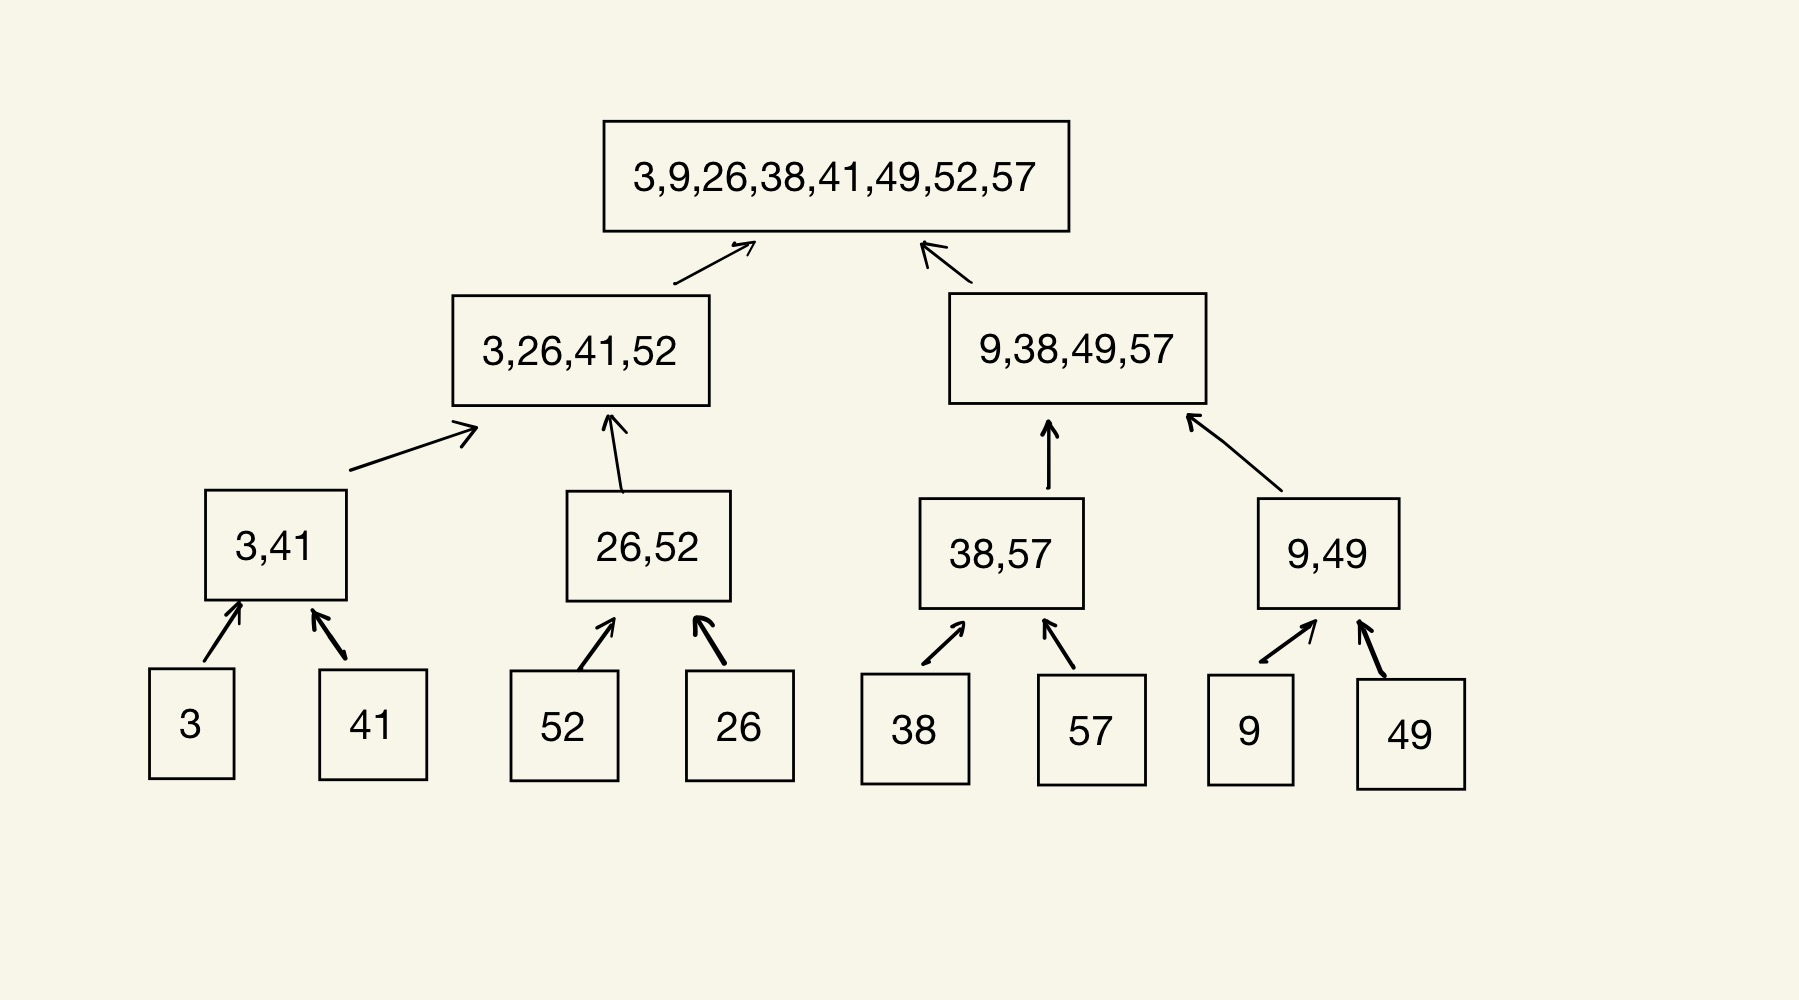
\includegraphics[scale=0.2]{sections/2/exercise2-3-1.jpeg}\\


\subti{2.3-2}
\begin{lstlisting}[language=Python,numbers=left,numberstyle=\normalsize]
MERGE(A,p,q,r):
    n1 = q - p + 1
    n2 = r - q
    let L[1 ... n1+1] and R[1 ... n2+1]
    for i = 1 to n1:
        L[i] = A[p + i - 1]
    for j = 1 to n2:
        R[j] = A[q + j]
    i = 1
    j = 1
    k = p
    while i < n1 and j < n2:
        if L[i] < R[j]:
            A[k] = L[i]
            i = i + 1
        else:
            A[k] = R[j]
            j = j + 1
        k = k + 1
    if i = n1:
        for t = j to n2:
            A[k] = R[j]
            j = j + 1
            k = k + 1
    else:
        for t = i to n1:
            A[k] = L[i]
            i = i + 1
            k = k + 1
MERGESORT(A,p,r):
    if p < r:
        q = [(p + r) / 2]
        MERGESORT(A,p,q)
        MERGESORT(A,q+1,r)
        MERGE(A,p,q,r)
\end{lstlisting}


\subti{2.3-3}\\
while $ n=2 $: $ T(2)=2=2\lg 2 $\\
while $ n=2^k , k>1 $:$ T(2^k)=2T(n/2)+n=(k-1)\cdot 2^k +2^k=k\cdot 2^k=n\lg n$\\
Q.E.D.\\


\subti{2.3-4}
\begin{align}
T(n)=\begin{dcases}
    1 & if n = 1\\
    T(n - 1) + n - 1 & if n > 1
\end{dcases}\notag
\end{align}


\subti{2.3-5}\\
binary search:
\begin{lstlisting}[language=Python,numbers=left,numberstyle=\normalsize]
binarysearch1(A,v):
    head = 1
    tail = A.length
    while head < tail :
        mid = (head + tail) / 2
        if v < A[mid]:
            tail = mid - 1
        else:
            head = mid
    return mid
\end{lstlisting}
Through binary searching, we guarantee that $ v $ occurs 
in an array that is half the length of the previous array.\\


\subti{2.3-6}\\
No. Even if we can use a binary search to simplify the searching part, 
the running time of moving $A[j]$ is still $\Theta(n^2)$